% Digital Logic Report Template
% Created: 2020-01-10, John Miller

%==========================================================
%=========== Document Setup  ==============================

% Formatting defined by class file
\documentclass[11pt]{article}

% ---- Document formatting ----
\usepackage[margin=1in]{geometry}	% Narrower margins
\usepackage{booktabs}				% Nice formatting of tables
\usepackage{graphicx}				% Ability to include graphics
\usepackage[section]{placeins}      % Stops floats from happening

%\setlength\parindent{0pt}	% Do not indent first line of paragraphs 
\usepackage[parfill]{parskip}		% Line space b/w paragraphs
%	parfill option prevents last line of pgrph from being fully justified

% Parskip package adds too much space around titles, fix with this
\RequirePackage{titlesec}
\titlespacing\section{0pt}{8pt plus 4pt minus 2pt}{3pt plus 2pt minus 2pt}
\titlespacing\subsection{0pt}{4pt plus 4pt minus 2pt}{-2pt plus 2pt minus 2pt}
\titlespacing\subsubsection{0pt}{2pt plus 4pt minus 2pt}{-6pt plus 2pt minus 2pt}

% ---- Hyperlinks ----
\usepackage[colorlinks=true,urlcolor=blue]{hyperref}	% For URL's. Automatically links internal references.

% ---- Code listings ----
\usepackage{listings} 					% Nice code layout and inclusion
\usepackage[usenames,dvipsnames]{xcolor}	% Colors (needs to be defined before using colors)

% Define custom colors for listings
\definecolor{listinggray}{gray}{0.98}		% Listings background color
\definecolor{rulegray}{gray}{0.7}			% Listings rule/frame color

% Style for Verilog
\lstdefinestyle{Verilog}{
	language=Verilog,					% Verilog
	backgroundcolor=\color{listinggray},	% light gray background
	rulecolor=\color{blue}, 			% blue frame lines
	frame=tb,							% lines above & below
	linewidth=\columnwidth, 			% set line width
	basicstyle=\small\ttfamily,	% basic font style that is used for the code	
	breaklines=true, 					% allow breaking across columns/pages
	tabsize=3,							% set tab size
	commentstyle=\color{gray},	% comments in italic 
	stringstyle=\upshape,				% strings are printed in normal font
	showspaces=false,					% don't underscore spaces
}

% How to use: \Verilog[listing_options]{file}
\newcommand{\Verilog}[2][]{%
	\lstinputlisting[style=Verilog,#1]{#2}
}




%======================================================
%=========== Body  ====================================
\begin{document}

\title{ELC 2137 Lab 08: 4-digit Display}
\author{Maddie Vorhies}

\maketitle


\section*{Summary}

My goal in this lab was to create a 4-digit display and add the ability to switch between hexadecimal and decimal (BCD) output on my Basys3 board. To do this, I used the sseg decoder, 11-bit circuit, and the mux2 from the previous lab. I modified the mux2 to include parameters in order to create flexible and reusable modules. After my mux2 was built, I created the mux4 and the anode decoder. The anode decoder allows you to switch between the four output digits. Once these were all built a created the sseg4 module to put all of these different part together. Lastly I created a manual that made the code much more organized and easier to read. I was then able to program my board and test the given inputs given in the lab. All of my test results were successful. My board successfully produced the correct outputs.



\section*{Results}

\begin{figure}[ht]\centering
	\begin{tabular}[ht]{c|c|c|c|c}
		Time (ns) & in0 & in1 & sel & output\\
		\midrule
		0 & 0110 & 1001 & 0 & 0110\\
		10 & 0110 & 1001 & 1 & 1001\\
		20 & 0011 & 1011 & 0 & 0011\\
		30 & 0011 & 1011 & 1 & 1011\\
		\bottomrule
	\end{tabular}\medskip
	
	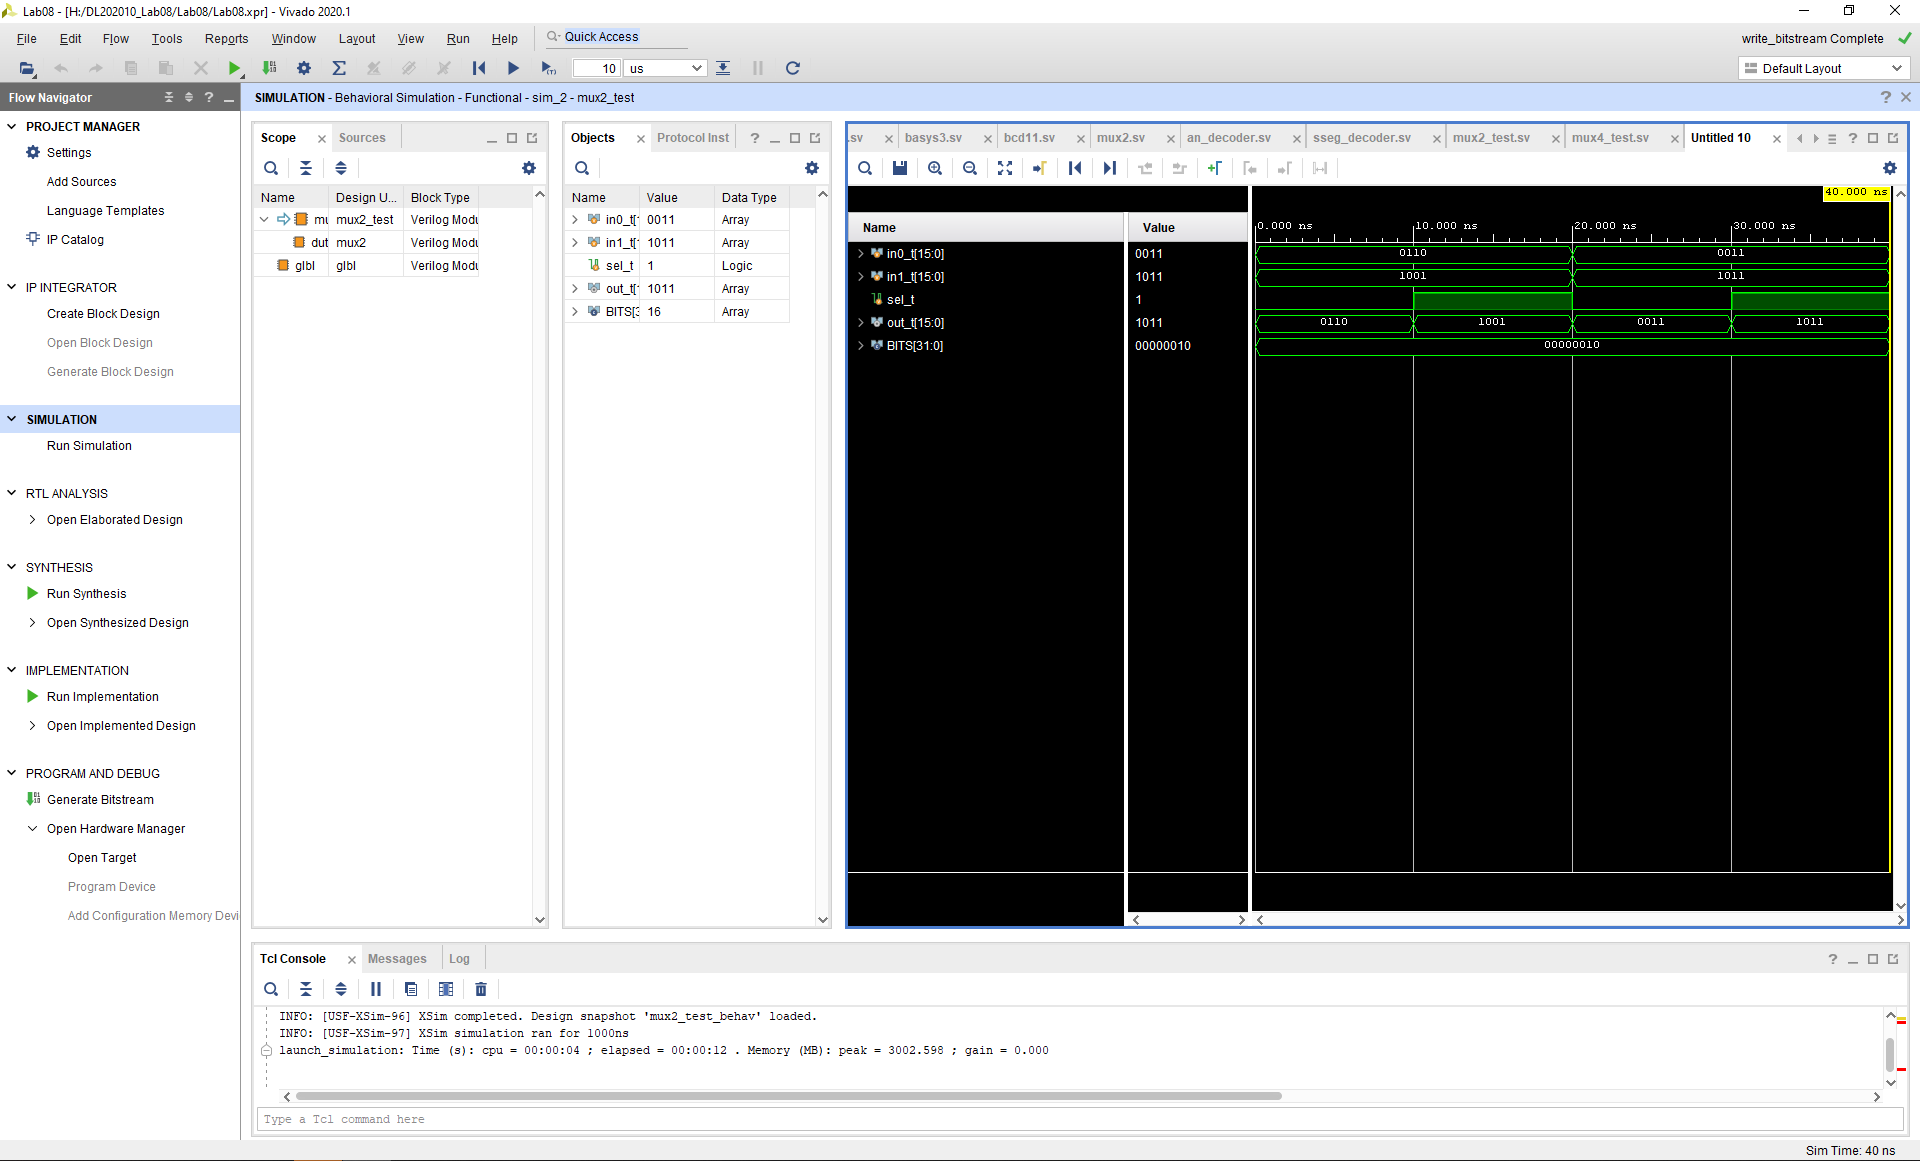
\includegraphics [width=1.0\textwidth,trim=640 550 10 135, clip]{mux2_sim}
	\caption{Simulation Waveform and ERT of mux2}
	\label{fig:sim_with_table}
	
\end{figure}


\section*{Code}

\Verilog{Lab08/systemverilog/mux2.sv}

\Verilog{Lab08/systemverilog/mux4.sv}

\Verilog{Lab08/systemverilog/an_decoder.sv}

\Verilog{Lab08/systemverilog/sseg4.sv}

\Verilog{Lab08/systemverilog/sseg4_manual.sv}


\end{document}
